\subsection{Modelo cliente-servidor}

La arquitectura de NFS responde a un modelo cliente-servidor. El servidor posee un sistema de archivos local, por ejemplo sobre XFS, ext4, ZFS u otro backend, y publica ciertos directorios para que otros equipos puedan montarlos. A esos directorios publicados se los denomina \textbf{exports}. Del lado del cliente, el sistema operativo monta el recurso remoto dentro de su propio arbol de directorios, de modo que las aplicaciones pueden acceder al contenido sin conocer la ubicacion fisica real de los datos.

En sistemas Linux, la configuracion del servidor suele expresarse en \texttt{/etc/exports}. Alli se indica que rutas se exportan, que clientes pueden acceder y con que opciones. Desde la perspectiva de redes, esto muestra que NFS combina control de acceso por red con permisos del sistema de archivos: no alcanza con que el usuario tenga permisos UNIX si el host no esta autorizado a montar el recurso.

\begin{figure}[H]
    \centering
    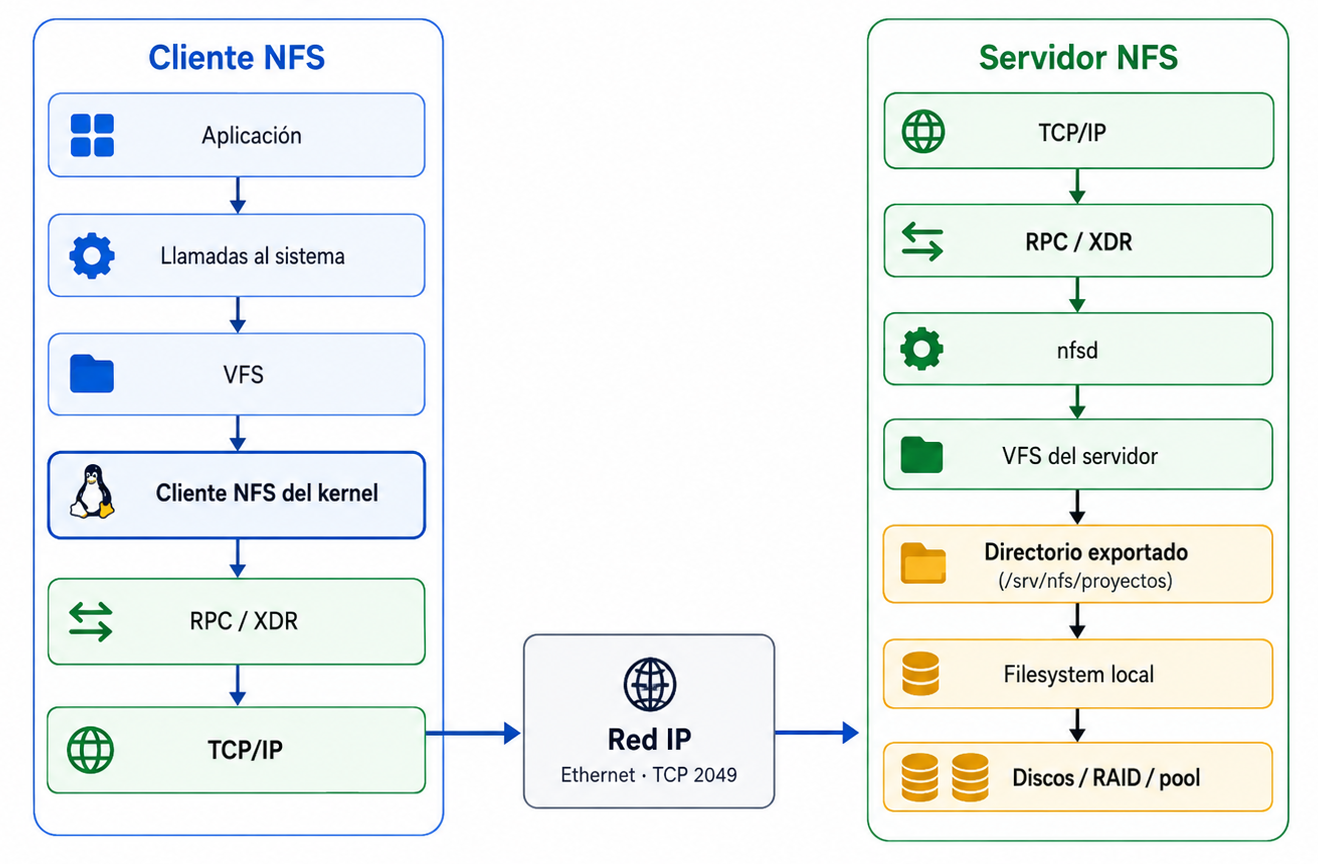
\includegraphics[width=0.95\textwidth]{img/nfs_01.png}
    \caption{Arquitectura cliente-servidor de NFS}
    \label{fig:nfs_arquitectura}
\end{figure}

\subsection{Integración con VFS, RPC y XDR}

La transparencia de NFS se logra mediante la integracion con la capa \textbf{VFS (Virtual File System)} del sistema operativo. VFS actua como una interfaz comun entre las aplicaciones y distintos tipos de sistemas de archivos. Cuando una aplicacion accede a un archivo local, VFS dirige la operacion hacia el modulo local. Cuando el archivo pertenece a un montaje NFS, VFS redirige la operacion hacia el cliente NFS del kernel, que genera una solicitud de red.

NFS utiliza \textbf{ONC RPC (Open Network Computing Remote Procedure Call)} para invocar operaciones remotas. En lugar de enviar bloques sin estructura, el cliente realiza llamadas como \texttt{LOOKUP}, \texttt{GETATTR}, \texttt{READ}, \texttt{WRITE} u \texttt{OPEN}. Para representar los datos de manera independiente de la arquitectura de CPU, RPC emplea \textbf{XDR (External Data Representation)}, una codificacion comun para enteros, cadenas y estructuras.

Desde el punto de vista de redes, NFS opera en la capa de aplicacion sobre TCP/IP. En despliegues modernos, el servicio NFS se asocia principalmente al \textbf{TCP 2049}. Esto es importante para diseñar ACLs, firewalls internos, monitoreo y segmentacion de trafico.

\subsection{NFSv3 y NFSv4 desde la red}

Una diferencia operativa importante entre NFSv3 y NFSv4 es la cantidad de servicios involucrados. En NFSv3, ademas de \texttt{nfsd} en el puerto 2049, suelen intervenir \texttt{rpcbind}, \texttt{mountd}, \texttt{lockd} y \texttt{statd}. Algunos pueden usar puertos dinamicos, lo que complica el filtrado en firewalls y el diagnostico en redes segmentadas.

NFSv4 simplifica este aspecto. Integra el montaje, el locking y la gestion de estado dentro del protocolo principal, reduciendo la dependencia de servicios externos. En un datacenter con VLANs, firewalls internos o microsegmentacion, esta simplificacion es una ventaja clara porque permite controlar el servicio principalmente con reglas sobre TCP 2049.

\begin{figure}[H]
    \centering
    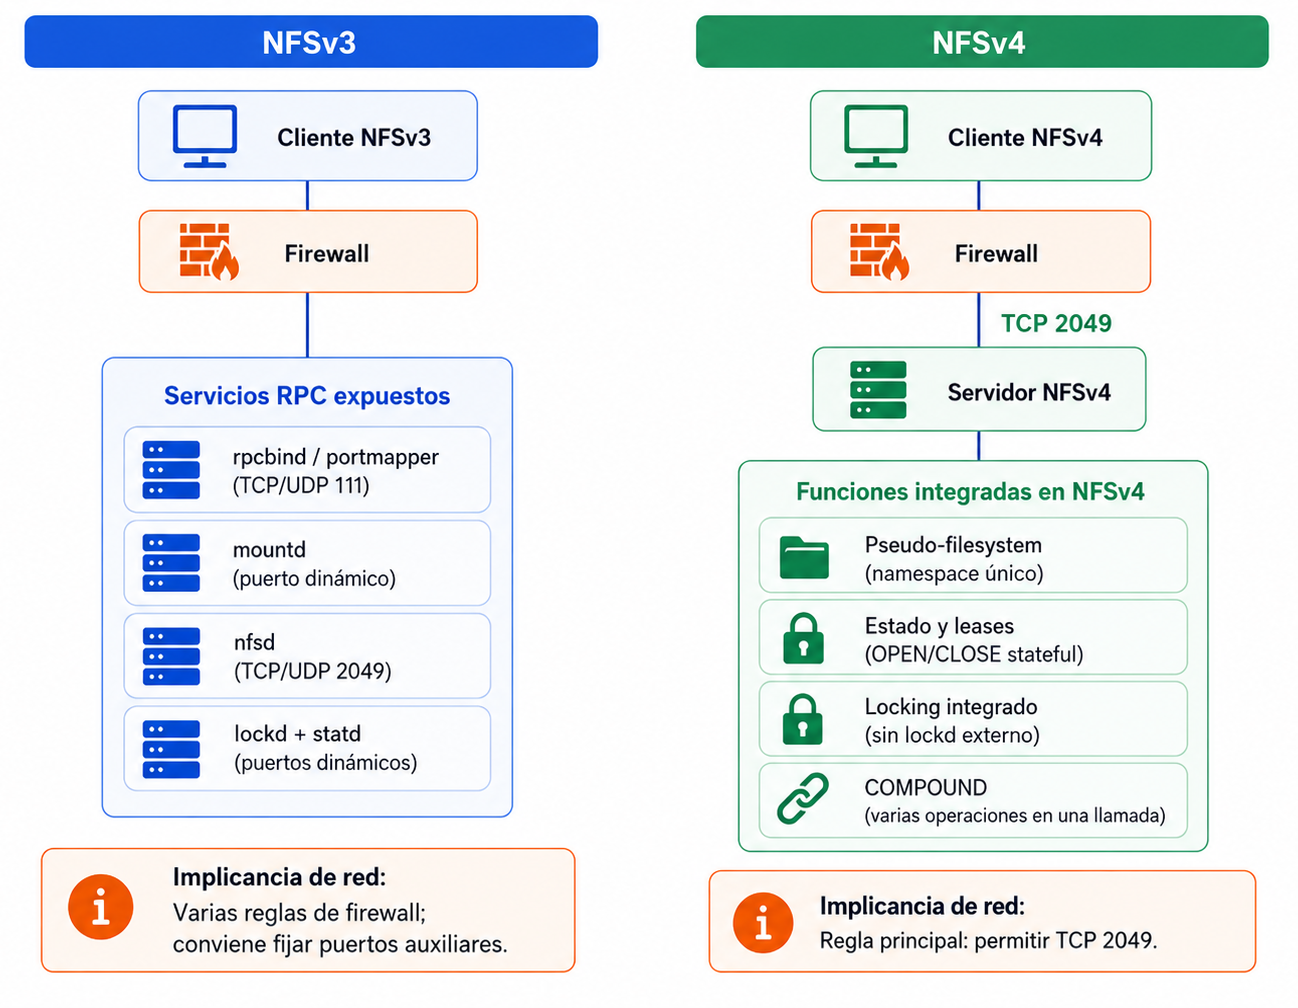
\includegraphics[width=0.95\textwidth]{img/nfs_02.png}
    \caption{NFSv3 frente a NFSv4}
    \label{fig:nfs_puertos}
\end{figure}

\subsection{Operaciones, caché y locking}

Cuando un cliente lee un archivo remoto, la aplicacion invoca una operacion comun de lectura. El kernel detecta que el archivo pertenece a un montaje NFS y genera una solicitud RPC de tipo \texttt{READ}. En una escritura, el cliente envia una solicitud \texttt{WRITE}; la forma en que el servidor confirma esa escritura depende de las politicas de durabilidad y de la cache disponible.

El cliente NFS mantiene cache local para reducir trafico de red y mejorar latencia percibida. Se cachean datos, atributos y entradas de directorio. La consistencia no es identica a un disco local: NFS suele usar una semantica \textbf{close-to-open}, donde un cierre propaga cambios relevantes y una apertura posterior valida atributos para detectar modificaciones.

Los permisos se basan en la semantica UNIX. En el modelo clasico \texttt{AUTH\_SYS}, cada solicitud incluye UID y GID, por lo que cliente y servidor deben tener identidades coherentes. El locking tambien depende de la version: en NFSv3 se apoya en servicios auxiliares, mientras que en NFSv4 forma parte del protocolo principal.
